\section{Methodology}\label{chapter:methodology}

This chapter presents the architecture, mathematical formulations, and training methodology of Sec-LogLLM, the proposed hybrid system for explainable log-based anomaly detection. The design rationale for each component is grounded in the research gaps identified in Chapter~\ref{chapter:lit-review}.

\subsection{System Overview}\label{sec:system-overview}

Sec-LogLLM is a hybrid architecture that combines a domain-specific encoder with a causal language model decoder through a novel explainability bottleneck. The system is designed to accept raw, unstructured log text as input and produce a structured JSON analysis containing three fields: a binary classification label (\texttt{Attack} or \texttt{Normal}), an optional MITRE ATT\&CK technique code (\texttt{mitre\_t\_code}), and a natural language reasoning string explaining the decision. Crucially, the system simultaneously produces per-log importance weights ($\alpha$ values) that identify which log lines in the input sequence drove the classification.

The architecture consists of three components arranged as a sequential pipeline:

\begin{enumerate}
    \item \textbf{SecBERT Encoder}: A cybersecurity-specialised BERT model (\texttt{jackaduma/SecBERT}) that processes each raw log line independently and produces a fixed-size embedding vector $\mathbf{h}_i \in \mathbb{R}^{768}$. Variable-length log sequences containing up to 128 lines are encoded into a padded tensor of shape $(B, T, 768)$, where $B$ is the batch size and $T$ is the maximum sequence length in the batch.

    \item \textbf{Alpha-Gated Projector}: A trainable module that serves two functions simultaneously. First, it linearly projects each 768-dimensional encoder embedding into the decoder's embedding space ($\mathbb{R}^{d_{\text{dec}}}$), bridging the dimensionality gap between the two models. Second, it computes a scalar importance weight $\alpha_i \in (0, 1)$ for each log line via a learned gating network, and multiplies the projected embedding by this weight. The output dimension of the projector is automatically set to match the decoder's hidden size during initialisation.

    \item \textbf{LLM Decoder}: A causal language model (\texttt{Qwen/Qwen2.5-3B-Instruct}) that receives a composite input embedding sequence and autoregressively generates the structured JSON output. The decoder is adapted to the security domain via Low-Rank Adaptation (LoRA) rather than full fine-tuning, preserving the model's general language capabilities while specialising its output behaviour.
\end{enumerate}

\begin{figure}[H]
    \centering
    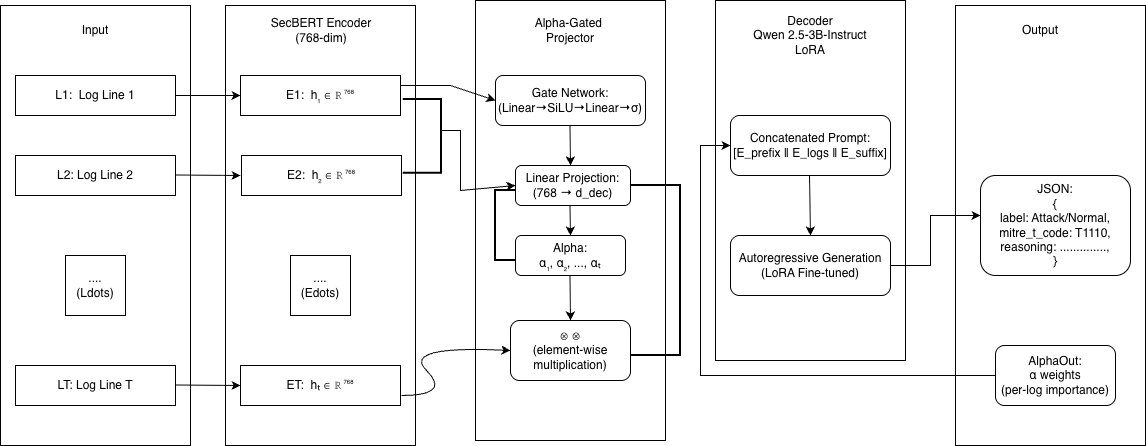
\includegraphics[width=\textwidth]{img/Ch3-dig1.drawio.png}
    \caption{Architecture of Sec-LogLLM. Raw log lines are encoded by SecBERT, weighted by the alpha-gating mechanism, and decoded by the LLM into a structured JSON analysis.}
    \label{fig:architecture}
\end{figure}

\subsubsection{Forward Pass}

During the forward pass, the three components are composed into a single end-to-end pipeline. Given a batch of raw log sequences, the system first encodes each log line through SecBERT to obtain pooled embeddings. These embeddings are then passed through the alpha-gated projector, which produces both the projected representations and the corresponding alpha weights.

The projected log embeddings are not passed to the decoder in isolation. Instead, they are sandwiched between two segments of tokenised text that form a structured prompt. The \textit{prefix} segment contains a system instruction that establishes the model's role as a Security Operations Centre (SOC) copilot, followed by a user-turn preamble introducing the log embeddings. The \textit{suffix} segment closes the user turn, specifies the desired JSON output format, and opens the assistant turn to begin generation. These text segments are converted into decoder-space embeddings using the decoder's own embedding layer.

The final input to the decoder is a concatenation of four embedding sequences along the sequence dimension:
\begin{equation}\label{eq:forward-concat}
    \mathbf{E}_{\text{input}} = [\mathbf{E}_{\text{prefix}} \; \| \; \mathbf{E}_{\text{logs}} \; \| \; \mathbf{E}_{\text{suffix}} \; \| \; \mathbf{E}_{\text{target}}]
\end{equation}
where $\mathbf{E}_{\text{prefix}}$ and $\mathbf{E}_{\text{suffix}}$ are the tokenised prompt embeddings, $\mathbf{E}_{\text{logs}}$ are the alpha-weighted projected log embeddings, and $\mathbf{E}_{\text{target}}$ contains the ground-truth response embeddings during training (omitted during inference). A corresponding attention mask is constructed to account for padding in variable-length sequences. During training, labels are set to $-100$ (ignored by the cross-entropy loss) for all positions except the target response tokens, ensuring the decoder only learns to generate the analysis output.

\subsubsection{Inference}

At inference time, the system operates identically through the encoding and projection stages, but the target embeddings are excluded from the concatenated input. The decoder then autoregressively generates up to 128 new tokens, which are decoded back to text using the decoder's tokeniser. The generated text is expected to be a valid JSON object conforming to the output schema. Alongside the generated text, the system returns the alpha weights $\alpha \in \mathbb{R}^{B \times T \times 1}$ for each log line, enabling analysts to inspect which events were deemed most relevant to the decision.

\subsection{SecBERT Encoder}\label{sec:encoder}

To extract rich semantic meaning from unstructured security logs before passing them to the LLM, the architecture employs a specialised encoding stage. Rather than using standard pre-trained models like BERT or RoBERTa, which are optimised for general English NLP tasks, Sec-LogLLM integrates \texttt{jackaduma/SecBERT}, a domain-specific BERT variant pre-trained extensively on cybersecurity text and system logs. Using a domain-specific encoder prevents the semantic dilution that occurs when generic tokenisers indiscriminately split complex identifiers (e.g., file paths, IP addresses, or registry keys) into meaninglessly small subwords.

\subsubsection{Input Processing and Pooling}

Raw log sequences are passed to the encoder in variable-length batches. Each individual log line $l_{i}$ within a sequence is independently tokenised. To balance computational efficiency with contextual capacity, the maximum sequence length per log line is capped at 256 tokens; any line exceeding this limit is truncated, while shorter lines are padded up to the batch maximum. 

Once tokenised, the log lines pass through the bidirectional Transformer layers of SecBERT. To reduce the sequence of token embeddings into a single fixed-size representation for the entire log line, the model extracts the embedding corresponding to the special \texttt{[CLS]} token from the final hidden state. Formally, for a given log line $l_i$, the encoding process yields a pooled embedding vector:
\begin{equation}\label{eq:encoder-pooling}
    \mathbf{h}_i = \text{SecBERT}(l_i)_{\texttt{[CLS]}} \quad \text{where} \quad \mathbf{h}_i \in \mathbb{R}^{768}
\end{equation}
This fixed-size representation $\mathbf{h}_i$ encapsulates the semantic state and syntax of the single event, making it suitable for subsequent mapping into the LLM's larger embedding space. 

\subsubsection{Update Strategy}

Unlike some parameter-efficient fine-tuning approaches that freeze early layers of an encoder to retain lower-level syntactic knowledge, Sec-LogLLM employs an all-or-nothing updating strategy across the entire encoder block depending on the training stage. During the initial alignment phase (Sec.~\ref{sec:training-strategy}), the entire SecBERT module is unfrozen, allowing the gradients to flow through all of its layers. This ensures that the encoder can learn to align its intermediate representations with the LLM's latent space. Once this alignment is complete, the entire encoder is explicitly frozen (requiring no gradients) during the final end-to-end generation phase, ensuring that the carefully aligned representations do not drift while the projector and LLM adapters are optimised for the final task.

\subsection{Alpha-Gating Mechanism}\label{sec:alpha-gating}

In standard transformer-based systems, passing encoder embeddings directly to a decoder via a simple linear projection achieves feature alignment but sacrifices interpretability. In the context of log-based anomaly detection, it is not sufficient for a model to simply flag a sequence of 128 logs as malicious; analysts require immediate evidence regarding exactly which log lines triggered the alert. While post-hoc explainability methods such as SHAP or LIME can identify these influential features, they require thousands of expensive perturbation-based inference passes per input. This latency is prohibitive for real-time Security Operations Centre (SOC) monitoring, and such methods often suffer from fidelity issues, producing approximations rather than faithful reflections of the model's true reasoning process.

To address this, Sec-LogLLM uses an \textit{Alpha-Gating Mechanism}—a learned computational bottleneck placed between the encoder and decoder. This mechanism intrinsically learns the importance of each log line during training and computes it directly during the forward pass, yielding faithful feature attribution with zero computational overhead at inference time.

\subsubsection{Gating Architecture}

The alpha-gating mechanism is implemented as a parallel branch augmenting the standard cross-modal linear projection. Given a 768-dimensional encoder embedding $\mathbf{h}_i \in \mathbb{R}^{d_{\text{enc}}}$ for the $i$-th log line, a standard approach simply maps it to the decoder's hidden dimension $d_{\text{dec}}$ via a linear projection:
\begin{equation}
    \tilde{\mathbf{z}}_i = \mathbf{W}_{\text{proj}} \mathbf{h}_i + \mathbf{b}_{\text{proj}}
\end{equation}
Optional regularisation steps such as LayerNorm and Dropout may be applied after the projection, though in the default configuration both are disabled. 

In the alpha-gated architecture, a secondary gating network independently computes a scalar weight $\alpha_i \in (0,1)$ representing the relevance of the specific log line. To capture complex relationships within the embedding space, the gating network is designed as a two-layer multi-layer perceptron (MLP) employing a SiLU (Sigmoid Linear Unit) activation function in the hidden layer.

Formally, the intermediate hidden representation $\mathbf{g}_i \in \mathbb{R}^{d_{\text{gate}}}$ (where $d_{\text{gate}} = 128$) and the scalar logit $s_i \in \mathbb{R}$ are computed as:
\begin{align}
    \mathbf{g}_i &= \text{SiLU}(\mathbf{W}_1 \mathbf{h}_i + \mathbf{b}_1) \label{eq:gate-hidden} \\
    s_i &= \mathbf{W}_2 \mathbf{g}_i + \mathbf{b}_2 \label{eq:gate-logit}
\end{align}
Here, $\mathbf{W}_1 \in \mathbb{R}^{128 \times d_{\text{enc}}}$, $\mathbf{W}_2 \in \mathbb{R}^{1 \times 128}$, and $\mathbf{b}_1, \mathbf{b}_2$ are learned bias terms.

To derive the final gating value $\alpha_i$, the raw logit $s_i$ is divided by a temperature scaling parameter $\tau$ (default $\tau = 1.0$) before passing through a sigmoid activation function:
\begin{equation}\label{eq:gate-alpha}
    \alpha_i = \sigma\left( \frac{s_i}{\tau} \right) = \frac{1}{1 + \exp(-s_i / \tau)}
\end{equation}
This gating value $\alpha_i$ is then element-wise multiplied with the projected embedding $\tilde{\mathbf{z}}_i$ to produce the final, alpha-weighted representation $\mathbf{z}_i$ that is passed to the LLM decoder:
\begin{equation}\label{eq:gate-final}
    \mathbf{z}_i = \alpha_i \cdot \tilde{\mathbf{z}}_i
\end{equation}

\subsubsection{Interpretability Properties}

The resulting $\alpha_i$ weights offer an \textit{intrinsic} explanation of the pipeline's behaviour by acting as a mathematically grounded attention map. Because $\mathbf{z}_i \approx \mathbf{0}$ when $\alpha_i \to 0$, log lines that the gate network determines to be task-irrelevant are effectively zeroed out, masking their semantic content from the decoder's self-attention layers. Conversely, log lines with $\alpha_i \to 1$ pass their full projected semantic information to the language model. 

Crucially, because the $\alpha_i$ values are computed natively inside the projector module, these importance scores are effortlessly extracted alongside the generated JSON response in a single forward pass. This bypasses the severe computational bottlenecks inherent to post-hoc strategies like SHAP, offering exact, unapproximated insight into the precise feature subset the unified pipeline relied upon to detect an anomaly.

\subsection{Training Objective: Alignment and Sparsity}\label{sec:training-objective}

The alpha-gating mechanism described in Section~\ref{sec:alpha-gating} requires a specialised loss function during the projector alignment phase (Stage 2). A naive approach would simply minimise the reconstruction error between the projected log embeddings and some target representation. However, without an explicit incentive to keep $\alpha$ values sparse, the gating network would learn to assign uniformly high importance to all log lines, rendering the explainability mechanism uninformative.

To enforce a ``need-to-know'' principle---where only genuinely relevant log lines receive high $\alpha$ values---the training objective combines two complementary terms. The first is a \textit{Mean Squared Error} (MSE) alignment loss that minimises the distance between the mean-pooled projected embeddings and the mean-pooled decoder-space target embeddings:
\begin{equation}\label{eq:mse-loss}
    \mathcal{L}_{\text{align}} = \text{MSE}\!\left( \frac{1}{T}\sum_{i=1}^{T} \mathbf{z}_i, \;\; \frac{1}{S}\sum_{j=1}^{S} \mathbf{e}_j^{\text{target}} \right)
\end{equation}
where $\mathbf{z}_i$ are the alpha-weighted projected log embeddings and $\mathbf{e}_j^{\text{target}}$ are the decoder-space embeddings of the ground-truth target response, with the summations producing sequence-level representations.

The second term is an $L_1$ sparsity penalty on the mean alpha values, which penalises the model for assigning unnecessary importance to log lines:
\begin{equation}\label{eq:l1-loss}
    \mathcal{L}_{\text{sparsity}} = \frac{1}{N} \sum_{i=1}^{N} |\alpha_i|
\end{equation}
where $N$ is the total number of log lines in the batch. The complete training objective for Stage 2 is therefore:
\begin{equation}\label{eq:total-loss}
    \mathcal{L}_{\text{total}} = \mathcal{L}_{\text{align}} + \lambda_{L_1} \cdot \mathcal{L}_{\text{sparsity}}
\end{equation}
The sparsity coefficient $\lambda_{L_1}$ controls the trade-off between alignment fidelity and interpretability. A default value of $\lambda_{L_1} = 0.01$ is used, which was determined through preliminary experiments to encourage meaningful sparsity without degrading alignment quality.

\subsection{Three-Stage Training Strategy}\label{sec:training-strategy}

Training the full Sec-LogLLM pipeline from scratch in a single pass would be unstable: the randomly initialised projector would inject noise into the decoder, while the decoder's gradients would disturb the encoder's pre-trained representations. To address this, the system is trained in three sequential stages, each with a distinct objective and a carefully chosen set of frozen and trainable parameters. Table~\ref{tab:training-stages} summarises the configuration of each stage.

\begin{table}[H]
\centering
\small
\begin{tabular}{|l|c|c|c|l|c|}
\hline
\textbf{Stage} & \textbf{Encoder} & \textbf{Projector} & \textbf{Decoder} & \textbf{Loss} & \textbf{LR} \\
\hline
1: Decoder SFT & Frozen & Frozen & LoRA trained & Cross-entropy & $2 \times 10^{-5}$ \\
2: Alignment & Trained & Trained & Frozen & $\mathcal{L}_{\text{total}}$ (Eq.~\ref{eq:total-loss}) & $2 \times 10^{-4}$ \\
3: End-to-End & Frozen & Trained & LoRA trained & Cross-entropy & $1 \times 10^{-4}$ \\
\hline
\end{tabular}
\caption{Summary of the three-stage training strategy. ``Frozen'' indicates all parameters have \texttt{requires\_grad=False}. ``LoRA trained'' indicates that only the low-rank adapter parameters are updated.}
\label{tab:training-stages}
\end{table}

\subsubsection{Stage 1: Decoder Adaptation (Supervised Fine-Tuning)}

The first stage adapts the pre-trained LLM decoder to the security domain and the desired output format before it interacts with the encoder or projector. At this stage, neither the SecBERT encoder nor the alpha-gated projector participates in training; both are frozen. The objective is to teach the decoder to produce well-structured JSON responses containing an attack classification label, a MITRE ATT\&CK technique code (where applicable), and a natural language reasoning string.

Rather than full fine-tuning, which would require updating all 3 billion parameters of the Qwen2.5-3B-Instruct model, Stage 1 employs Low-Rank Adaptation (LoRA). LoRA injects small, trainable low-rank matrices into specific layers of the transformer, dramatically reducing the number of trainable parameters while preserving the model's pre-trained knowledge. The LoRA configuration used is as follows:

\begin{itemize}
    \item \textbf{Rank} ($r$): 16
    \item \textbf{Alpha} ($\alpha_{\text{LoRA}}$): 32
    \item \textbf{Dropout}: 0.1
    \item \textbf{Target modules}: \texttt{q\_proj}, \texttt{k\_proj}, \texttt{v\_proj}, \texttt{o\_proj}, \texttt{gate\_proj}, \texttt{up\_proj}, \texttt{down\_proj}
\end{itemize}

The training data consists of individual log entries formatted as ChatML conversations, where the system message establishes the model's role as a security analyst, the user message presents a raw log line, and the assistant message contains the desired JSON response. The model is trained using the standard causal language modelling cross-entropy loss with a learning rate of $2 \times 10^{-5}$ over 3 epochs, with gradient accumulation across 4 steps per update.

\subsubsection{Stage 2: Projector Alignment}

With the decoder now capable of producing well-formatted security analyses, Stage 2 establishes the communication channel between the SecBERT encoder and the decoder through the alpha-gated projector. The Stage 1 LoRA adapter is loaded into the decoder, and the entire decoder (including the adapter weights) is frozen. The encoder and projector are both unfrozen and trained jointly.

The objective is to align the projected encoder representations with the decoder's latent space using the composite loss function defined in Section~\ref{sec:training-objective}. To compute the alignment loss, the sequence of projected log embeddings $\mathbf{z}_1, \ldots, \mathbf{z}_T$ is mean-pooled along the sequence dimension to produce a single vector, and similarly, the decoder-space target embeddings are mean-pooled. The MSE between these two pooled representations, combined with the $L_1$ sparsity penalty on the alpha values, drives the encoder and projector to learn representations that are both compatible with the decoder's expectations and interpretably sparse.

This stage trains for 2 epochs with a learning rate of $2 \times 10^{-4}$, a batch size of 8, and gradient accumulation over 4 steps. The AdamW optimiser is used with $\beta = (0.9, 0.95)$ and weight decay of 0.01. Upon completion, both the encoder and projector state dictionaries are saved as a checkpoint.

\subsubsection{Stage 3: End-to-End Fine-Tuning}

The final stage jointly optimises the projector and the decoder's LoRA adapters to maximise task performance. The Stage 1 LoRA adapter and Stage 2 encoder/projector checkpoint are both loaded. The encoder is then re-frozen to prevent the aligned representations from drifting, while the projector remains trainable to allow further refinement.

To selectively unfreeze only the LoRA parameters within the decoder (rather than all decoder weights), the system scans all named parameters and sets \texttt{requires\_grad=True} exclusively for those whose names contain the substring ``lora''. All other decoder parameters remain frozen.

The loss function in this stage is the standard causal language modelling cross-entropy loss, as computed by the decoder model itself. This directly optimises the quality of the generated JSON output, including classification accuracy, MITRE ATT\&CK code assignment, and reasoning quality. Training runs for 1 epoch with a learning rate of $1 \times 10^{-4}$, a batch size of 4, and gradient accumulation over 8 steps. The final checkpoint saves the encoder, projector, and LoRA adapter states.

\subsection{Datasets}\label{sec:datasets}

% TODO: Describe each dataset used in training and evaluation.

\subsubsection{AIT Log Data Set v1.1}

% TODO: Primary multi-host training/validation dataset.
% - Source description, size (~244MB training, ~60MB validation)
% - Log types covered, labelling methodology
% - Reference: src/utils/ait_v1_parser.py, data/ait_v1.1/

\subsubsection{OpenSSH Dataset}

% TODO: Single-host generalisation evaluation dataset.
% - Purpose: test cross-dataset generalisation
% - Size (~4MB), log types
% - Reference: src/utils/openssh_parser.py, data/openssh/

\subsubsection{BGL Dataset}

% TODO: Out-of-distribution evaluation dataset.
% - Purpose: hallucination testing (non-security logs)
% - Expected behaviour: model should NOT assign MITRE codes
% - Reference: data/processed/ood_bgl.jsonl

\subsection{Evaluation Metrics}\label{sec:evaluation-metrics}

% TODO: Define each metric used to evaluate Sec-LogLLM.

\subsubsection{Classification Performance}

% TODO: Standard metrics.
% - F1 Score (macro and weighted), precision, recall
% - Confusion matrix
% - Reference: src/evaluation/metrics.py (compute_classification_metrics)

\subsubsection{Fidelity Score}

% TODO: The key XAI evaluation metric.
% - Definition: does removing the highest-α log change the prediction?
% - Process: run model → get prediction + alphas → remove highest-α log → re-run → compare
% - Fidelity = 1.0 if prediction changes, 0.0 otherwise; averaged across test set
% - Reference: src/evaluation/metrics.py (compute_fidelity_score)

\subsubsection{Hallucination Rate}

% TODO: OOD reliability metric.
% - Definition: rate of assigning MITRE codes to normal/non-security events
% - Hallucination Rate = (hallucinated MITRE codes) / (total predictions)
% - Evaluated on BGL dataset
% - Reference: src/evaluation/metrics.py (compute_hallucination_rate)

\subsubsection{Alpha Sparsity}

% TODO: Interpretability quality metric.
% - Definition: fraction of alpha weights below threshold
% - Alpha Sparsity = (1/N) Σ 𝟙(α < 0.1)
% - Higher sparsity indicates model is focusing on fewer, more relevant logs
